\documentclass{standalone}
\usepackage{standalone}

\begin{document}
\section{Support Vector Machine}

SVM is a supervised learning algorithm which is used analyze classification and regression analysis data. SVM is normally used to classify data into 2 categories. It performs better than Gaussian Naive Bayes. In SVM, the training data is plotted in the hyperspace and a hyper plane is drawn which separates the data into 2 categories as widely as possible. This hyper plane is called SVM.

\begin{figure}[h]
				\centering
				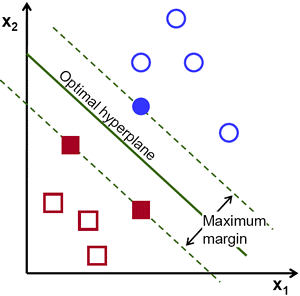
\includegraphics[scale=1.5]{./img/svm}
				\caption{Basic Support Vector Machine} \label{fig:mapComp}
\end{figure}

If there exists multiple class in the training data set, then multiple SVM is drawn to classify them. 
If the number of feature is too large or number of data set is too large then SVM does not perform well. 

\end{document}